\documentclass[10pt,a4paper,draft]{article}
\usepackage[utf8x]{inputenc}
\usepackage{ucs}
\usepackage[english]{babel}
\usepackage{multirow}
\usepackage{rotating}
\author{Lukáš Petrovický}
\title{RAS2012: Competition Entry}
\begin{document}

\maketitle

\begin{abstract}
This article describes an entry to the 2012 RAS Problem Solving Competition, concerning dispatching on multi-track territories. The entry is based on the Drools Planner, a Java-based solver. On a reasonably recent computer, the resulting algorithm is able to produce feasible results within a minute and has been fine-tuned to provide best results in under 3 minutes. Source code to the entry is open source and well documented.
\end{abstract}

\section{Introduction}

\section{Describing the solution}

\section{Implementation}

\section{Achieved results}

Running the algorithm described above 20 times over each data set, we have compiled a set of results, see Table \ref{table:results}. All these were reached within 3 minutes in a single-threaded run, using Intel i7 Q820 processor running Fedora 17 and 2 GB of heap space inside Java 7 runtime environment.

\begin{table}
\caption{Solution performance per data set.}
\begin{tabular}{c||c|c|c|c|c|c}
\hline \hline
    & Best    & Q1      & Q2      & Q3      & Worst   & Std. dev. \\ 
\hline
TOY & \$808   & \$960   & \$1210  & \$1210  & \$1210  & 164 \\ 
\hline 
1   & \$1435  & \$1695  & \$1930  & \$2856  & \$5612  & 1219 \\ 
\hline 
2   & \$8097  & \$10364 & \$14865 & \$16177 & \$22486 & 4088 \\ 
\hline 
3   & \$10617 & \$13247 & \$15367 & \$17307 & \$21384 & 2986 \\ 
\end{tabular} 
\label{table:results}
\end{table}

Please note that via the benchmarking functionality of Drools Planner (see above), users may be able to fine-tune the algorithm to be focused either on providing better solutions or on faster turnaround times.

For statistics of the resolved systems, see tables \ref{table:TOY-808.tex}, \ref{table:RDS1-1435.tex}, \ref{table:RDS2-8097.tex} and \ref{table:RDS3-10617.tex} respectively. 

\section{Conclusion}

\appendix

\section{Resolved systems}

In this section, we show the best solutions reached for each data set. 

\begin{sidewaystable}
\centering
\footnotesize
\caption{Statistics for resolved system ``RAS DATA SET TOY'', costing \$808.}
\begin{tabular}{c||c|c||c|c|c|c|c||c|c|c}
  \hline \hline
  &
  Unpref. & 
  Delay &
  Node &
  When &
  SA &
  +/- &
  Pty &
  TWT &
  +/- &
  Pty \\
      \hline
      \multirow{2}{*}{A1} &
      \multirow{2}{*}{0} &
      \multirow{2}{*}{1260} &
      6 &
      4260 &
      2400 &
        -1860 &
        0 &
      \multirow{2}{*}{8700} &
        \multirow{2}{*}{2640} &
        \multirow{2}{*}{0}
      \\
      \cline{4-8}
       &
       &
       &
      12 &
      6060 &
      4800 &
        -1260 &
        0 &
      
         &
        
      \\
      \hline
      \multirow{2}{*}{B1} &
      \multirow{2}{*}{0} &
      \multirow{2}{*}{3480} &
      6 &
      6283.16 &
      -3000 &
        -9283.16 &
        115 &
      \multirow{2}{*}{4800} &
        \multirow{2}{*}{-3903.328} &
        \multirow{2}{*}{0}
      \\
      \cline{4-8}
       &
       &
       &
      0 &
      8703.328 &
      5400 &
        -3303.328 &
        0 &
      
         &
        
      \\
      \hline
      \multirow{2}{*}{C1} &
      \multirow{2}{*}{0} &
      \multirow{2}{*}{0} &
      6 &
      2400 &
      3000 &
        600 &
        0 &
      \multirow{2}{*}{7200} &
        \multirow{2}{*}{2400} &
        \multirow{2}{*}{0}
      \\
      \cline{4-8}
       &
       &
       &
      12 &
      4800 &
      6000 &
        1200 &
        0 &
      
         &
        
      \\
\end{tabular}
\label{table:TOY-808.tex} 
\end{sidewaystable}

\begin{sidewaystable}
\footnotesize
\caption{Statistics for resolved system ``RAS DATA SET 1'', costing \$1435.}
\centering
\begin{tabular}{c||c|c||c|c|c|c|c||c|c|c}
  \hline \hline
  &
  Unpref. & 
  Delay &
  Node &
  When &
  SA &
  +/- &
  Pty &
  TWT &
  +/- &
  Pty \\
      \hline
      \multirow{2}{*}{A1} &
      \multirow{2}{*}{0} &
      \multirow{2}{*}{0} &
      37 &
      3082.5 &
      3600 &
        517.5 &
        0 &
      \multirow{2}{*}{5400} &
        \multirow{2}{*}{-1003.5} &
        \multirow{2}{*}{0}
      \\
      \cline{4-8}
       &
       &
       &
      39 &
      6403.5 &
      7800 &
        1396.5 &
        0 &
      
         &
        
      \\
      \hline
      \multirow{2}{*}{A2} &
      \multirow{2}{*}{6} &
      \multirow{2}{*}{1680} &
      37 &
      6244.742 &
      7800 &
        1555.258 &
        0 &
      \multirow{2}{*}{9000} &
        \multirow{2}{*}{-1569.166} &
        \multirow{2}{*}{0}
      \\
      \cline{4-8}
       &
       &
       &
      39 &
      10569.166 &
      12000 &
        1430.834 &
        0 &
      
         &
        
      \\
      \hline
      \multirow{2}{*}{B1} &
      \multirow{2}{*}{11} &
      \multirow{2}{*}{0} &
      37 &
      10486.282 &
      12600 &
        2113.718 &
        0 &
      \multirow{2}{*}{13800} &
        \multirow{2}{*}{-153.266} &
        \multirow{2}{*}{0}
      \\
      \cline{4-8}
       &
       &
       &
      0 &
      13953.266 &
      17400 &
        3446.734 &
        0 &
      
         &
        
      \\
      \hline
      \multirow{2}{*}{B2} &
      \multirow{2}{*}{0} &
      \multirow{2}{*}{0} &
      37 &
      13898.112 &
      15600 &
        1701.888 &
        0 &
      \multirow{2}{*}{16800} &
        \multirow{2}{*}{-448.224} &
        \multirow{2}{*}{0}
      \\
      \cline{4-8}
       &
       &
       &
      39 &
      17248.224 &
      19800 &
        2551.776 &
        0 &
      
         &
        
      \\
      \hline
      \multirow{2}{*}{B3} &
      \multirow{2}{*}{4} &
      \multirow{2}{*}{1380} &
      37 &
      40517.661 &
      40200 &
        -317.661 &
        0 &
      \multirow{2}{*}{42000} &
        \multicolumn{2}{c}{\multirow{2}{*}{N/A}}
      \\
      \cline{4-8}
       &
       &
       &
      39 &
      44126.528 &
      45000 &
        \multicolumn{2}{|c||}{N/A} &
      
        
      \\
      \hline
      \multirow{2}{*}{C1} &
      \multirow{2}{*}{0} &
      \multirow{2}{*}{0} &
      37 &
      17598 &
      19200 &
        1602 &
        0 &
      \multirow{2}{*}{21600} &
        \multirow{2}{*}{282} &
        \multirow{2}{*}{0}
      \\
      \cline{4-8}
       &
       &
       &
      39 &
      21318 &
      24600 &
        3282 &
        0 &
      
         &
        
      \\
      \hline
      \multirow{2}{*}{C2} &
      \multirow{2}{*}{13} &
      \multirow{2}{*}{120} &
      37 &
      25086.431 &
      27000 &
        1913.569 &
        0 &
      \multirow{2}{*}{28800} &
        \multirow{2}{*}{-21.004} &
        \multirow{2}{*}{0}
      \\
      \cline{4-8}
       &
       &
       &
      39 &
      28821.004 &
      33000 &
        4178.996 &
        0 &
      
         &
        
      \\
      \hline
      \multirow{2}{*}{D1} &
      \multirow{2}{*}{11} &
      \multirow{2}{*}{0} &
      37 &
      26478.851 &
      29400 &
        2921.149 &
        0 &
      \multirow{2}{*}{31200} &
        \multirow{2}{*}{152.585} &
        \multirow{2}{*}{0}
      \\
      \cline{4-8}
       &
       &
       &
      0 &
      31047.415 &
      36600 &
        5552.585 &
        0 &
      
         &
        
      \\
      \hline
      \multirow{2}{*}{D2} &
      \multirow{2}{*}{5} &
      \multirow{2}{*}{6240} &
      37 &
      25254.463 &
      21600 &
        -3654.463 &
        0 &
      \multirow{2}{*}{23400} &
        \multirow{2}{*}{-6339.89} &
        \multirow{2}{*}{0}
      \\
      \cline{4-8}
       &
       &
       &
      0 &
      29739.89 &
      28200 &
        -1539.89 &
        0 &
      
         &
        
      \\
      \hline
      \multirow{2}{*}{D3} &
      \multirow{2}{*}{0} &
      \multirow{2}{*}{0} &
      37 &
      32868.738 &
      35400 &
        2531.262 &
        0 &
      \multirow{2}{*}{37200} &
        \multirow{2}{*}{415.34} &
        \multirow{2}{*}{0}
      \\
      \cline{4-8}
       &
       &
       &
      0 &
      36784.66 &
      41400 &
        4615.34 &
        0 &
      
         &
        
      \\
      \hline
      \multirow{2}{*}{E1} &
      \multirow{2}{*}{0} &
      \multirow{2}{*}{9180} &
      37 &
      42657 &
      36000 &
        -6657 &
        0 &
      \multirow{2}{*}{39000} &
        \multicolumn{2}{c}{\multirow{2}{*}{N/A}}
      \\
      \cline{4-8}
       &
       &
       &
      39 &
      70515 &
      44400 &
        \multicolumn{2}{|c||}{N/A} &
      
        
      \\
      \hline
      \multirow{2}{*}{F1} &
      \multirow{2}{*}{0} &
      \multirow{2}{*}{0} &
      37 &
      50831.998 &
      57600 &
        \multicolumn{2}{|c||}{N/A} &
      \multirow{2}{*}{63000} &
        \multicolumn{2}{c}{\multirow{2}{*}{N/A}}
      \\
      \cline{4-8}
       &
       &
       &
      0 &
      61734.853 &
      75000 &
        \multicolumn{2}{|c||}{N/A} &
      
        
      \\
\end{tabular}
\label{table:RDS1-1435.tex} 
\end{sidewaystable}
\begin{sidewaystable}
\footnotesize
\caption{Statistics for resolved system ``RAS DATA SET 2'', costing \$8097.}
\centering
\begin{tabular}{c||c|c||c|c|c|c|c||c|c|c}
  \hline \hline
  &
  Unpref. & 
  Delay &
  Node &
  When &
  SA &
  +/- &
  Pty &
  TWT &
  +/- &
  Pty \\
      \hline
      \multirow{2}{*}{A1} &
      \multirow{2}{*}{7} &
      \multirow{2}{*}{11520} &
      37 &
      14245.5 &
      3600 &
        -10645.5 &
        191 &
      \multirow{2}{*}{5400} &
        \multirow{2}{*}{-11452.5} &
        \multirow{2}{*}{13}
      \\
      \cline{4-8}
       &
       &
       &
      39 &
      16852.5 &
      7800 &
        -9052.5 &
        102 &
      
         &
        
      \\
      \hline
      \multirow{2}{*}{A2} &
      \multirow{2}{*}{8} &
      \multirow{2}{*}{4740} &
      37 &
      14845.583 &
      11400 &
        -3445.583 &
        0 &
      \multirow{2}{*}{12600} &
        \multirow{2}{*}{-4922.851} &
        \multirow{2}{*}{0}
      \\
      \cline{4-8}
       &
       &
       &
      39 &
      17522.851 &
      15600 &
        -1922.851 &
        0 &
      
         &
        
      \\
      \hline
      \multirow{2}{*}{A3} &
      \multirow{2}{*}{7} &
      \multirow{2}{*}{0} &
      37 &
      16798.5 &
      18000 &
        1201.5 &
        0 &
      \multirow{2}{*}{19800} &
        \multirow{2}{*}{67.5} &
        \multirow{2}{*}{0}
      \\
      \cline{4-8}
       &
       &
       &
      39 &
      19732.5 &
      22200 &
        2467.5 &
        0 &
      
         &
        
      \\
      \hline
      \multirow{2}{*}{A4} &
      \multirow{2}{*}{7} &
      \multirow{2}{*}{720} &
      37 &
      35800.967 &
      31800 &
        -4000.967 &
        0 &
      \multirow{2}{*}{39000} &
        \multirow{2}{*}{-802.881} &
        \multirow{2}{*}{0}
      \\
      \cline{4-8}
       &
       &
       &
      0 &
      39802.881 &
      36600 &
        -3202.881 &
        0 &
      
         &
        
      \\
      \hline
      \multirow{2}{*}{B1} &
      \multirow{2}{*}{9} &
      \multirow{2}{*}{3960} &
      37 &
      10904.466 &
      4800 &
        -6104.466 &
        0 &
      \multirow{2}{*}{9600} &
        \multirow{2}{*}{-4774.578} &
        \multirow{2}{*}{0}
      \\
      \cline{4-8}
       &
       &
       &
      39 &
      14374.578 &
      9000 &
        -5374.578 &
        0 &
      
         &
        
      \\
      \hline
      \multirow{2}{*}{B2} &
      \multirow{2}{*}{11} &
      \multirow{2}{*}{840} &
      37 &
      32278.125 &
      26400 &
        -5878.125 &
        0 &
      \multirow{2}{*}{35400} &
        \multirow{2}{*}{-838.125} &
        \multirow{2}{*}{0}
      \\
      \cline{4-8}
       &
       &
       &
      39 &
      36238.125 &
      31200 &
        -5038.125 &
        0 &
      
         &
        
      \\
      \hline
      \multirow{2}{*}{B3} &
      \multirow{2}{*}{8} &
      \multirow{2}{*}{120} &
      37 &
      7433.144 &
      11400 &
        3966.856 &
        0 &
      \multirow{2}{*}{10800} &
        \multirow{2}{*}{-59.575} &
        \multirow{2}{*}{0}
      \\
      \cline{4-8}
       &
       &
       &
      0 &
      10859.575 &
      16800 &
        5940.425 &
        0 &
      
         &
        
      \\
      \hline
      \multirow{2}{*}{C1} &
      \multirow{2}{*}{6} &
      \multirow{2}{*}{960} &
      37 &
      36873.005 &
      26400 &
        -10473.005 &
        181 &
      \multirow{2}{*}{39000} &
        \multirow{2}{*}{-1407.472} &
        \multirow{2}{*}{0}
      \\
      \cline{4-8}
       &
       &
       &
      39 &
      40407.472 &
      31800 &
        -8607.472 &
        78 &
      
         &
        
      \\
      \hline
      \multirow{2}{*}{C2} &
      \multirow{2}{*}{10} &
      \multirow{2}{*}{0} &
      37 &
      198 &
      0 &
        -198 &
        0 &
      \multirow{2}{*}{3600} &
        \multirow{2}{*}{30} &
        \multirow{2}{*}{0}
      \\
      \cline{4-8}
       &
       &
       &
      39 &
      3570 &
      5400 &
        1830 &
        0 &
      
         &
        
      \\
      \hline
      \multirow{2}{*}{C3} &
      \multirow{2}{*}{8} &
      \multirow{2}{*}{1020} &
      37 &
      23070.001 &
      20400 &
        -2670.001 &
        0 &
      \multirow{2}{*}{25200} &
        \multirow{2}{*}{-2217.003} &
        \multirow{2}{*}{0}
      \\
      \cline{4-8}
       &
       &
       &
      0 &
      27417.003 &
      25800 &
        -1617.003 &
        0 &
      
         &
        
      \\
      \hline
      \multirow{2}{*}{D1} &
      \multirow{2}{*}{0} &
      \multirow{2}{*}{0} &
      37 &
      40306.5 &
      43800 &
        3493.5 &
        0 &
      \multirow{2}{*}{44400} &
        \multicolumn{2}{c}{\multirow{2}{*}{N/A}}
      \\
      \cline{4-8}
       &
       &
       &
      39 &
      45781.5 &
      51000 &
        \multicolumn{2}{|c||}{N/A} &
      
        
      \\
      \hline
      \multirow{2}{*}{D2} &
      \multirow{2}{*}{0} &
      \multirow{2}{*}{2340} &
      37 &
      1855.382 &
      3600 &
        1744.618 &
        0 &
      \multirow{2}{*}{6600} &
        \multirow{2}{*}{-2123.07} &
        \multirow{2}{*}{0}
      \\
      \cline{4-8}
       &
       &
       &
      39 &
      8723.07 &
      9600 &
        876.93 &
        0 &
      
         &
        
      \\
      \hline
      \multirow{2}{*}{E1} &
      \multirow{2}{*}{16} &
      \multirow{2}{*}{300} &
      37 &
      4952.184 &
      6600 &
        1647.816 &
        0 &
      \multirow{2}{*}{9600} &
        \multirow{2}{*}{-261.275} &
        \multirow{2}{*}{0}
      \\
      \cline{4-8}
       &
       &
       &
      39 &
      9861.275 &
      14400 &
        4538.725 &
        0 &
      
         &
        
      \\
      \hline
      \multirow{2}{*}{E2} &
      \multirow{2}{*}{0} &
      \multirow{2}{*}{2400} &
      37 &
      3534.858 &
      1800 &
        -1734.858 &
        0 &
      \multirow{2}{*}{7200} &
        \multirow{2}{*}{-2426.294} &
        \multirow{2}{*}{0}
      \\
      \cline{4-8}
       &
       &
       &
      0 &
      9626.294 &
      10800 &
        1173.706 &
        0 &
      
         &
        
      \\
      \hline
      \multirow{2}{*}{E3} &
      \multirow{2}{*}{0} &
      \multirow{2}{*}{43200} &
      37 &
      77389.713 &
      9000 &
        \multicolumn{2}{|c||}{N/A} &
      \multirow{2}{*}{12000} &
        \multicolumn{2}{c}{\multirow{2}{*}{N/A}}
      \\
      \cline{4-8}
       &
       &
       &
      0 &
      85085.14 &
      18000 &
        \multicolumn{2}{|c||}{N/A} &
      
        
      \\
      \hline
      \multirow{2}{*}{E4} &
      \multirow{2}{*}{22} &
      \multirow{2}{*}{0} &
      37 &
      27075.742 &
      30000 &
        2924.258 &
        0 &
      \multirow{2}{*}{32400} &
        \multirow{2}{*}{-91.404} &
        \multirow{2}{*}{0}
      \\
      \cline{4-8}
       &
       &
       &
      0 &
      32491.404 &
      37800 &
        5308.596 &
        0 &
      
         &
        
      \\
      \hline
      \multirow{2}{*}{F1} &
      \multirow{2}{*}{0} &
      \multirow{2}{*}{22140} &
      37 &
      47408.18 &
      29400 &
        \multicolumn{2}{|c||}{N/A} &
      \multirow{2}{*}{33600} &
        \multicolumn{2}{c}{\multirow{2}{*}{N/A}}
      \\
      \cline{4-8}
       &
       &
       &
      39 &
      55438.362 &
      41400 &
        \multicolumn{2}{|c||}{N/A} &
      
        
      \\
      \hline
      \multirow{2}{*}{F2} &
      \multirow{2}{*}{0} &
      \multirow{2}{*}{34560} &
      37 &
      56180.573 &
      30000 &
        \multicolumn{2}{|c||}{N/A} &
      \multirow{2}{*}{36000} &
        \multicolumn{2}{c}{\multirow{2}{*}{N/A}}
      \\
      \cline{4-8}
       &
       &
       &
      0 &
      69886.29 &
      51000 &
        \multicolumn{2}{|c||}{N/A} &
      
        
      \\
\end{tabular}
\label{table:RDS2-8097.tex} 
\end{sidewaystable}
\begin{sidewaystable}
\footnotesize
\caption{Statistics for resolved system ``RAS DATA SET 3'', costing \$10617.}
\centering
\begin{tabular}{c||c|c||c|c|c|c|c||c|c|c}
  \hline \hline
  &
  Unpref. & 
  Delay &
  Node &
  When &
  SA &
  +/- &
  Pty &
  TWT &
  +/- &
  Pty \\
      \hline
      \multirow{2}{*}{A1} &
      \multirow{2}{*}{7} &
      \multirow{2}{*}{0} &
      37 &
      967.5 &
      2400 &
        1432.5 &
        0 &
      \multirow{2}{*}{4200} &
        \multirow{2}{*}{298.5} &
        \multirow{2}{*}{0}
      \\
      \cline{4-8}
       &
       &
       &
      39 &
      3901.5 &
      6000 &
        2098.5 &
        0 &
      
         &
        
      \\
      \hline
      \multirow{2}{*}{A2} &
      \multirow{2}{*}{0} &
      \multirow{2}{*}{1260} &
      37 &
      2185.715 &
      2400 &
        214.285 &
        0 &
      \multirow{2}{*}{4200} &
        \multirow{2}{*}{-726.863} &
        \multirow{2}{*}{0}
      \\
      \cline{4-8}
       &
       &
       &
      0 &
      4926.863 &
      6600 &
        1673.137 &
        0 &
      
         &
        
      \\
      \hline
      \multirow{2}{*}{A3} &
      \multirow{2}{*}{7} &
      \multirow{2}{*}{0} &
      37 &
      21384.003 &
      22800 &
        1415.997 &
        0 &
      \multirow{2}{*}{24000} &
        \multirow{2}{*}{-775.721} &
        \multirow{2}{*}{0}
      \\
      \cline{4-8}
       &
       &
       &
      0 &
      24775.721 &
      27000 &
        2224.279 &
        0 &
      
         &
        
      \\
      \hline
      \multirow{2}{*}{A4} &
      \multirow{2}{*}{32} &
      \multirow{2}{*}{4320} &
      37 &
      40607.461 &
      33600 &
        -7007.461 &
        0 &
      \multirow{2}{*}{39000} &
        \multicolumn{2}{c}{\multirow{2}{*}{N/A}}
      \\
      \cline{4-8}
       &
       &
       &
      0 &
      43492.881 &
      38400 &
        \multicolumn{2}{|c||}{N/A} &
      
        
      \\
      \hline
      \multirow{2}{*}{A5} &
      \multirow{2}{*}{6} &
      \multirow{2}{*}{4815} &
      37 &
      36697.5 &
      32400 &
        -4297.5 &
        0 &
      \multirow{2}{*}{34200} &
        \multirow{2}{*}{-5521.5} &
        \multirow{2}{*}{0}
      \\
      \cline{4-8}
       &
       &
       &
      39 &
      39721.5 &
      36600 &
        -3121.5 &
        0 &
      
         &
        
      \\
      \hline
      \multirow{1}{*}{B1} &
      \multirow{1}{*}{0} &
      \multirow{1}{*}{0} &
      0 &
      1838.337 &
      1800 &
        -38.337 &
        0 &
      \multirow{1}{*}{1200} &
        \multirow{1}{*}{-638.337} &
        \multirow{1}{*}{0}
      \\
      \hline
      \multirow{1}{*}{B2} &
      \multirow{1}{*}{0} &
      \multirow{1}{*}{0} &
      39 &
      3240.208 &
      4800 &
        1559.792 &
        0 &
      \multirow{1}{*}{3000} &
        \multirow{1}{*}{-240.208} &
        \multirow{1}{*}{0}
      \\
      \hline
      \multirow{2}{*}{B3} &
      \multirow{2}{*}{4} &
      \multirow{2}{*}{4740} &
      37 &
      7747.488 &
      -3000 &
        -10747.488 &
        197 &
      \multirow{2}{*}{6000} &
        \multirow{2}{*}{-5519.129} &
        \multirow{2}{*}{0}
      \\
      \cline{4-8}
       &
       &
       &
      39 &
      11519.129 &
      1800 &
        -9719.129 &
        139 &
      
         &
        
      \\
      \hline
      \multirow{2}{*}{B4} &
      \multirow{2}{*}{12} &
      \multirow{2}{*}{14400} &
      37 &
      43207.716 &
      16800 &
        \multicolumn{2}{|c||}{N/A} &
      \multirow{2}{*}{32400} &
        \multicolumn{2}{c}{\multirow{2}{*}{N/A}}
      \\
      \cline{4-8}
       &
       &
       &
      0 &
      46634.147 &
      21600 &
        \multicolumn{2}{|c||}{N/A} &
      
        
      \\
      \hline
      \multirow{1}{*}{C1} &
      \multirow{1}{*}{0} &
      \multirow{1}{*}{1020} &
      0 &
      4362.853 &
      6000 &
        1637.147 &
        0 &
      \multirow{1}{*}{4200} &
        \multirow{1}{*}{-162.853} &
        \multirow{1}{*}{0}
      \\
      \hline
      \multirow{2}{*}{C2} &
      \multirow{2}{*}{0} &
      \multirow{2}{*}{5880} &
      37 &
      9246.431 &
      0 &
        -9246.431 &
        113 &
      \multirow{2}{*}{7200} &
        \multirow{2}{*}{-6387.861} &
        \multirow{2}{*}{0}
      \\
      \cline{4-8}
       &
       &
       &
      39 &
      13587.861 &
      6000 &
        -7587.861 &
        21 &
      
         &
        
      \\
      \hline
      \multirow{2}{*}{C3} &
      \multirow{2}{*}{20} &
      \multirow{2}{*}{7440} &
      37 &
      33148.656 &
      30000 &
        -3148.656 &
        0 &
      \multirow{2}{*}{37200} &
        \multicolumn{2}{c}{\multirow{2}{*}{N/A}}
      \\
      \cline{4-8}
       &
       &
       &
      0 &
      45070.536 &
      36000 &
        \multicolumn{2}{|c||}{N/A} &
      
        
      \\
      \hline
      \multirow{2}{*}{D1} &
      \multirow{2}{*}{6} &
      \multirow{2}{*}{7380} &
      37 &
      11009.995 &
      4200 &
        -6809.995 &
        0 &
      \multirow{2}{*}{7800} &
        \multirow{2}{*}{-7576.144} &
        \multirow{2}{*}{0}
      \\
      \cline{4-8}
       &
       &
       &
      39 &
      15376.144 &
      10200 &
        -5176.144 &
        0 &
      
         &
        
      \\
      \hline
      \multirow{2}{*}{D2} &
      \multirow{2}{*}{0} &
      \multirow{2}{*}{0} &
      37 &
      40247.997 &
      42000 &
        1752.003 &
        0 &
      \multirow{2}{*}{43800} &
        \multicolumn{2}{c}{\multirow{2}{*}{N/A}}
      \\
      \cline{4-8}
       &
       &
       &
      39 &
      45315.685 &
      48000 &
        \multicolumn{2}{|c||}{N/A} &
      
        
      \\
      \hline
      \multirow{2}{*}{E1} &
      \multirow{2}{*}{0} &
      \multirow{2}{*}{43200} &
      37 &
      95431.432 &
      10200 &
        \multicolumn{2}{|c||}{N/A} &
      \multirow{2}{*}{13200} &
        \multicolumn{2}{c}{\multirow{2}{*}{N/A}}
      \\
      \cline{4-8}
       &
       &
       &
      0 &
      147296.58 &
      19200 &
        \multicolumn{2}{|c||}{N/A} &
      
        
      \\
      \hline
      \multirow{2}{*}{E2} &
      \multirow{2}{*}{0} &
      \multirow{2}{*}{1380} &
      37 &
      15867 &
      18000 &
        2133 &
        0 &
      \multirow{2}{*}{21000} &
        \multirow{2}{*}{-1539} &
        \multirow{2}{*}{0}
      \\
      \cline{4-8}
       &
       &
       &
      39 &
      22539 &
      26400 &
        3861 &
        0 &
      
         &
        
      \\
      \hline
      \multirow{2}{*}{E3} &
      \multirow{2}{*}{0} &
      \multirow{2}{*}{0} &
      37 &
      18760.912 &
      21000 &
        2239.088 &
        0 &
      \multirow{2}{*}{24000} &
        \multirow{2}{*}{375.814} &
        \multirow{2}{*}{0}
      \\
      \cline{4-8}
       &
       &
       &
      39 &
      23624.186 &
      28800 &
        5175.814 &
        0 &
      
         &
        
      \\
      \hline
      \multirow{2}{*}{E4} &
      \multirow{2}{*}{12} &
      \multirow{2}{*}{164} &
      37 &
      38248 &
      40800 &
        2552 &
        0 &
      \multirow{2}{*}{43800} &
        \multicolumn{2}{c}{\multirow{2}{*}{N/A}}
      \\
      \cline{4-8}
       &
       &
       &
      39 &
      44928 &
      49800 &
        \multicolumn{2}{|c||}{N/A} &
      
        
      \\
      \hline
      \multirow{2}{*}{F1} &
      \multirow{2}{*}{0} &
      \multirow{2}{*}{43200} &
      37 &
      97662.855 &
      18000 &
        \multicolumn{2}{|c||}{N/A} &
      \multirow{2}{*}{23400} &
        \multicolumn{2}{c}{\multirow{2}{*}{N/A}}
      \\
      \cline{4-8}
       &
       &
       &
      0 &
      108627.424 &
      34800 &
        \multicolumn{2}{|c||}{N/A} &
      
        
      \\
      \hline
      \multirow{2}{*}{F2} &
      \multirow{2}{*}{0} &
      \multirow{2}{*}{13740} &
      37 &
      58413 &
      37200 &
        \multicolumn{2}{|c||}{N/A} &
      \multirow{2}{*}{42000} &
        \multicolumn{2}{c}{\multirow{2}{*}{N/A}}
      \\
      \cline{4-8}
       &
       &
       &
      39 &
      79929 &
      51000 &
        \multicolumn{2}{|c||}{N/A} &
      
        
      \\
\end{tabular}
\label{table:RDS3-10617.tex} 
\end{sidewaystable}

\section{Visualizations}

\begin{figure}
\centering
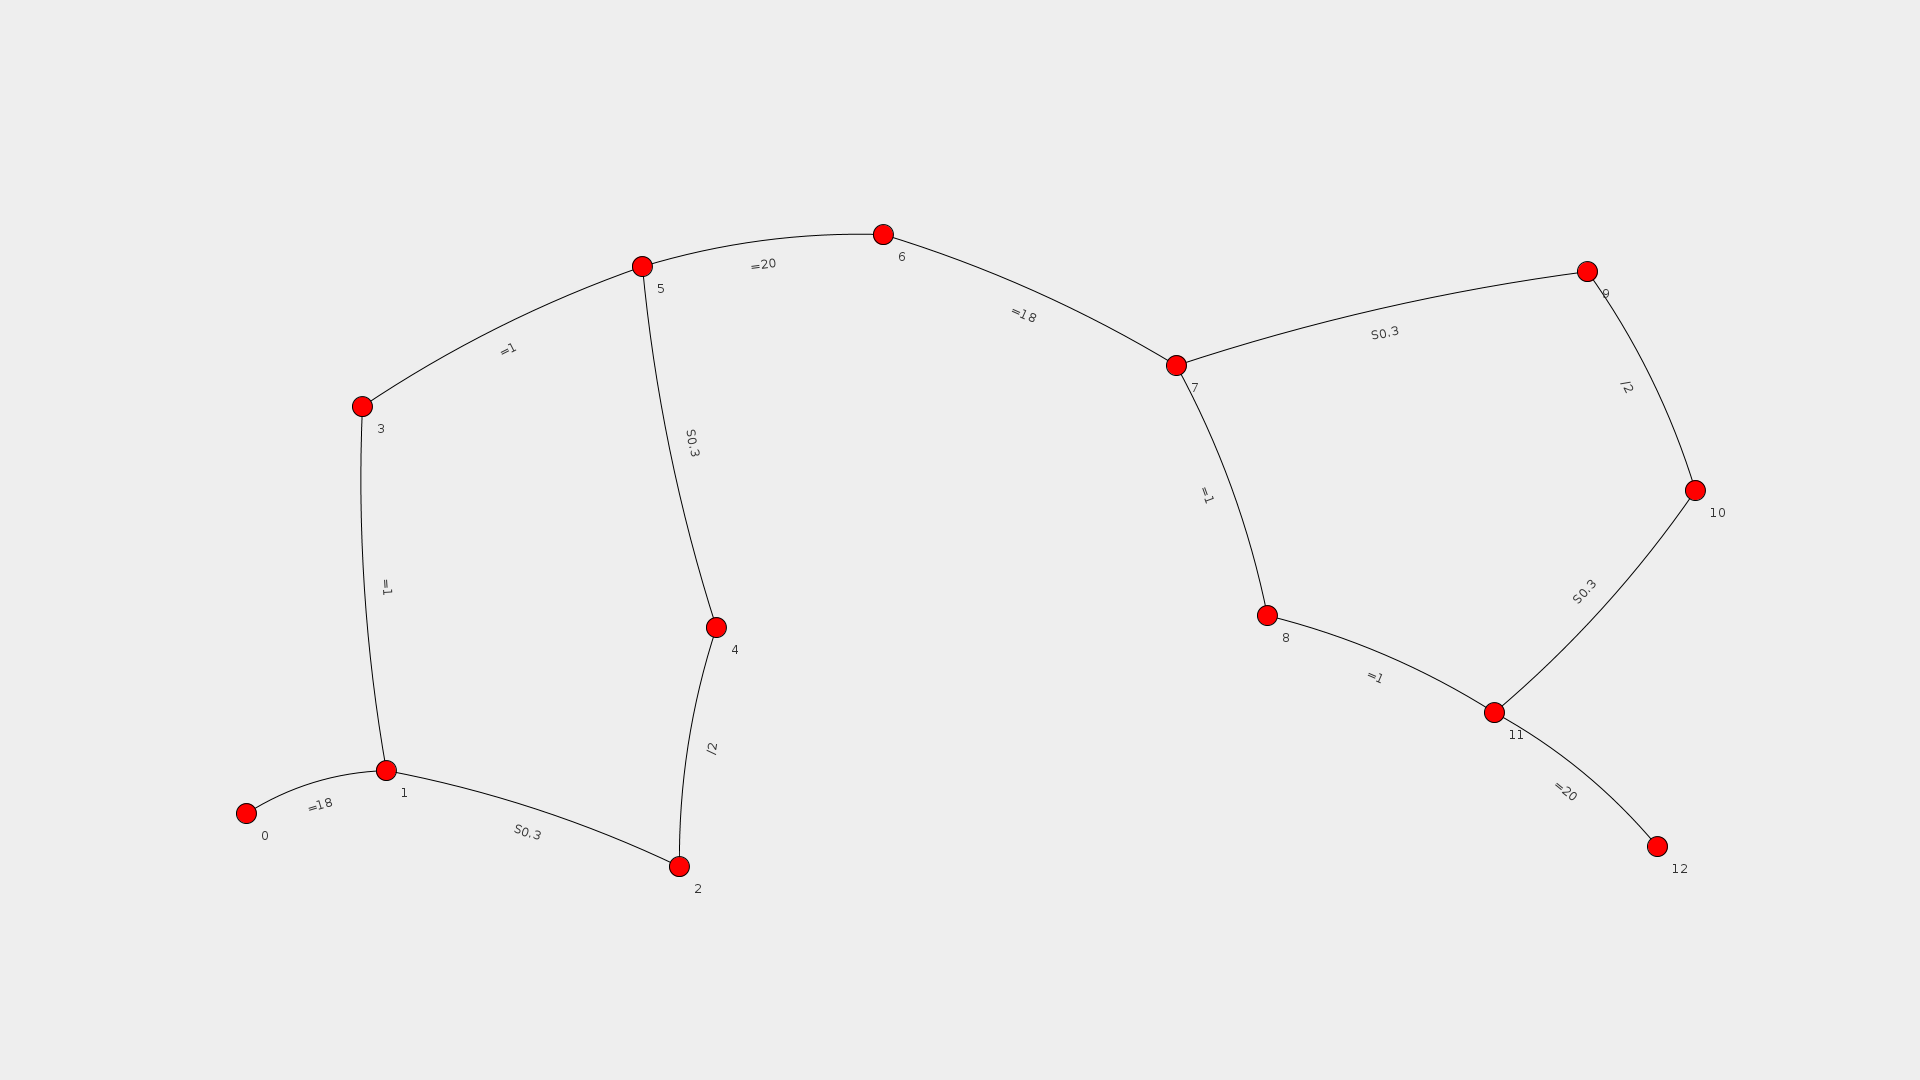
\includegraphics[width=150mm,angle=90]{solution.png}
\caption{RAS DATA SET TOY example territory. Undirected graph, arcs have descriptions.}
\end{figure}

\begin{figure}
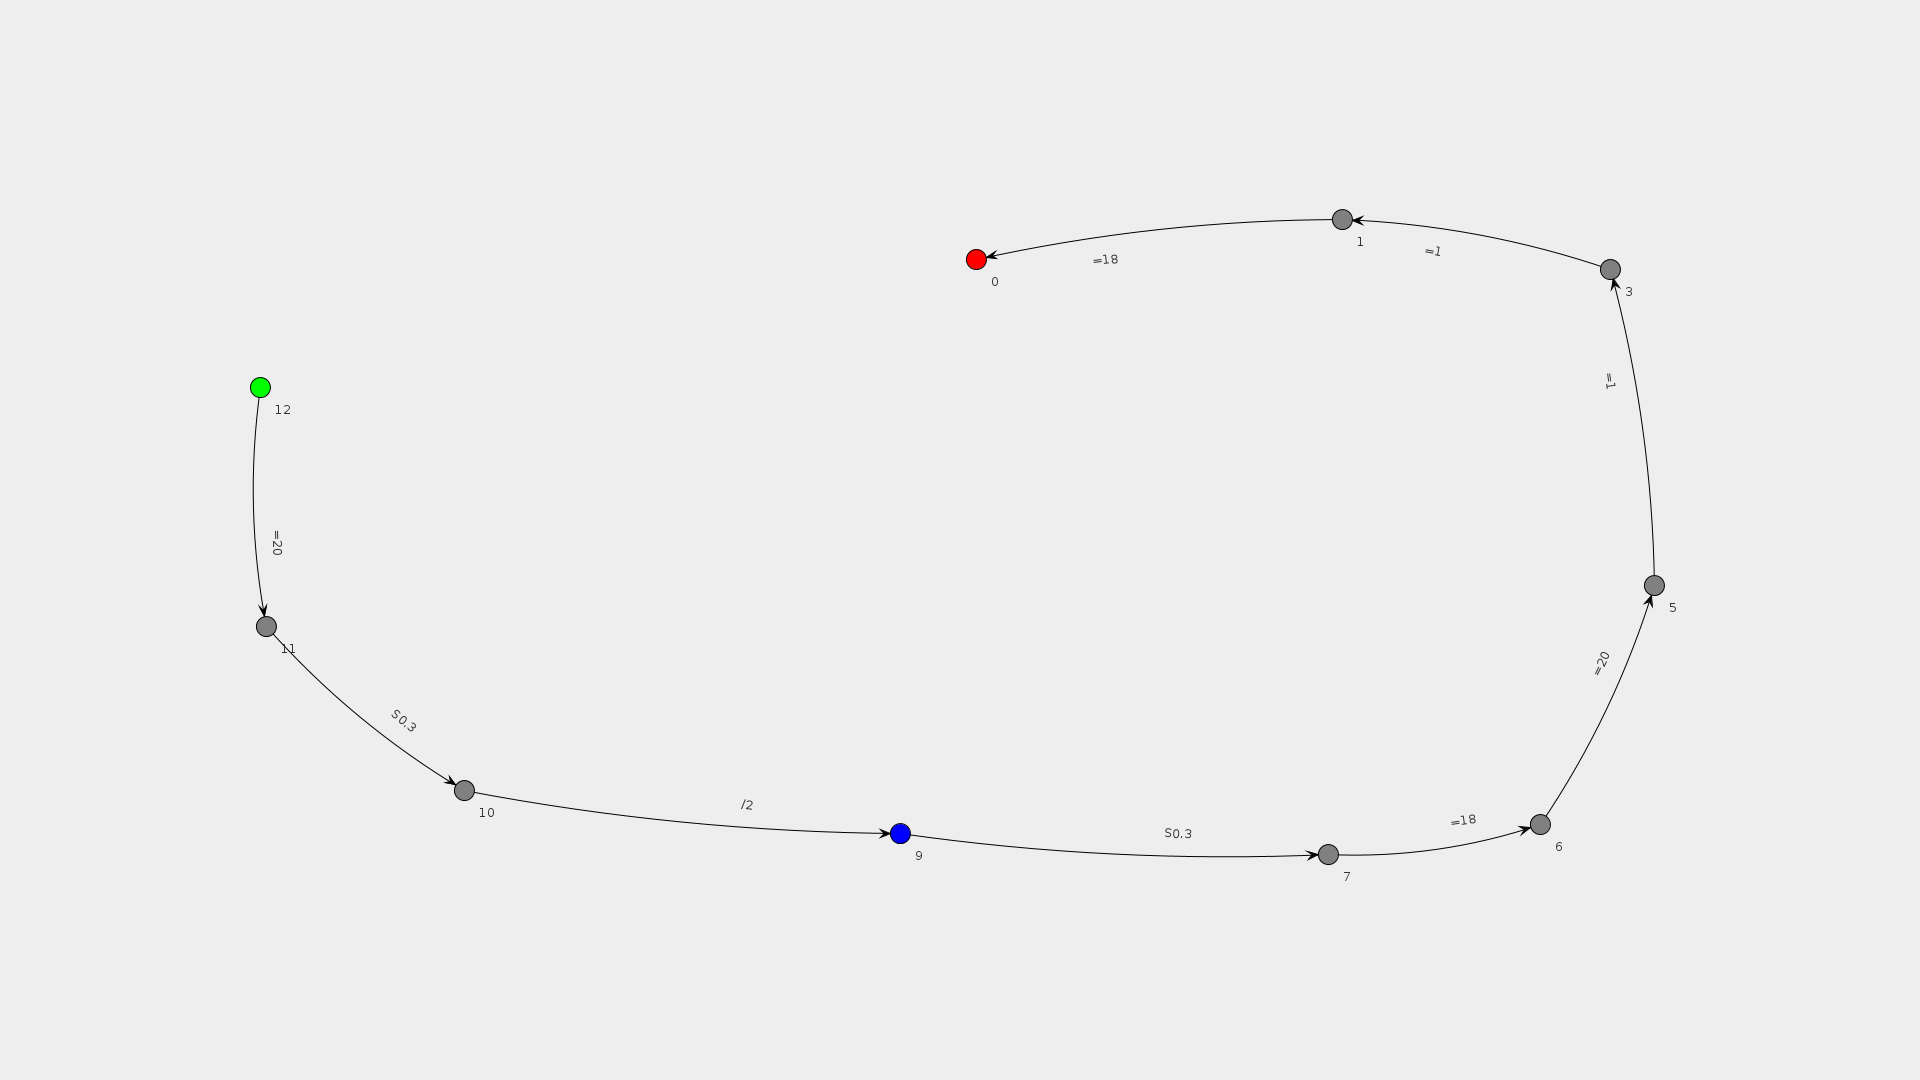
\includegraphics[width=150mm,angle=90]{B1.png}
\centering
\caption{RAS DATA SET TOY example, route of Train B1. Directed graph where green marks the origin, red the destination and blue is where the train is allowed to wait.}
\end{figure}

In this section, we show examples of visualizations that the solution is capable of providing. These visualizations have been rendered on the fly using the JUNG library\footnote{Java Universal Network/Graph framework, http://jung.sourceforge.net}.

\end{document}
